\documentclass[main.tex]{subfiles}
\begin{document}


\chapter{Double beta decay}
 

%\begin{flushright}
%\textit{Nothing contributes so much to tranquillize the mind \\
%as a steady purpose, a point on which the soul \\
%can focus its intellectual eye.}\\
%Mary Shelley, \textit{Frankenstein}.
%\end{flushright} 


\NI Since the neutrino existence prediction in 1930 and their first detection in 1956, many works have been realized to understand their properties. One of the more important achievements being the discovery of their oscillations, proving their non-zero mass which is a first indication of physics beyond Standard Model. 


\bigskip


\NI There are still remaining questions in neutrino physics including their nature and how they acquire their masses. Since it has been proved that the observation of the neutrinoless double beta decay necessarily involves Majorana neutrino, the search for this hypothetical decay is one of the most active research topic in neutrino physics. Its observation will give access of their Majorana nature and may give access to their absolute mass scale.


\bigskip


\NI Before to discuss the neutrinoless double beta decay in Section~\ref{sec:0NeutrinoDBD}, some elements about simple beta decay and double beta decay are introduced in Sections~\ref{sec:betaDecay} and~\ref{sec:2NeutrinoDBD}. The different detector technologies and the status of the search for neutrinoless double beta decay are presented in Section~\ref{sec:DBDexperiment} and~\ref{sec:StatusDBD}.


\section{Beta decay}\label{sec:betaDecay}


\NI Beta ($\beta$) decay is a radioactive decay which transmutes a nucleus to a different element. This decay is mediated by the weak interaction and is always accompanied by a neutrino or antineutrino emission. There are three separate forms :


\bigskip


\NI $\boldsymbol{\beta^-}$ \textbf{decay}, in which a neutron converts to a proton, an electron, and a antineutrino are emitted :
\begin{equation}
\text{n} \rightarrow \text{p} + \text{e}^- + \bar{\nu}_\text{e}
\end{equation}


\bigskip


\NI $\boldsymbol{\beta^+}$ \textbf{decay}, in which a proton converts to a neutron, an positron, and a neutrino are emitted :
\begin{equation}
\text{p} \rightarrow \text{n} + \text{e}^+ + \nu_\text{e}
\end{equation} 


\bigskip 

 
\NI \textbf{Electron capture (EC)}, in which an atomic electron is captured by its nucleus, resulting in the emission of a neutrino :
\begin{equation}
\text{p} + \text{e}^- \rightarrow \text{n} + \nu_{\text{e}}
\end{equation} 
 

\NI In $\beta^-$ and $\beta^+$ decays, the energy is shared between the $\beta$-particle and the neutrino or the antineutrino. This is not the case in electron captures where the emitted neutrino is monoenergetic. After an electron capture, the captured electron leaves a hole in the atomic orbital. The reorganisation of the remaining electrons is accompanied by a cascade of photons and/or Auger electron emissions. For the isotopes where the $\beta^+$ decay is possible, a competition exists with the electron capture process.


\bigskip


\NI The $\beta$ decays can only occur if the mass of the daughter nucleus, $\mathcal{M}$(A,Z$_\text{f}$), is lower than the mother nucleus, $\mathcal{M}$(A,Z$_\text{i}$), where A is the number of nucleons and Z is the atomic number.  


\bigskip


\NI All $\beta$ decays involve emission of particle and loss of energy, $\beta$ decay can only occur if the initial mass of the nucleus with A~nucleons and Z~protons, $\mathcal{M}$(A,Z$_\text{i}$), is greater than the final nucleus mass, $\mathcal{M}$(A,Z$_\text{f}$) : $\mathcal{M} \text{(A,Z}_\text{i}) > \mathcal{M} \text{(A,Z}_\text{f})$.


\bigskip


\NI As shown in Figure~\ref{WeizsackerParabola}, the $\beta$ decays (a) $\rightarrow$ (b) and (b) $\rightarrow$ (c) are allowed. Isotopes such as (c) are not completely stable but they can not decay by $\beta$ emission. To reach a stable state, they can undergo a neutrino double beta decay (2$\nu\beta\beta$). Note that it is theorically possible for the isotope (a) to directly decay to (c) by a 2$\nu\beta\beta$~decay, but this decay would not be observed since the decay rate of $\beta$~decay is far much shorter than 2$\nu\beta\beta$~decay.





\begin{equation}
\text{m} = \text{Z}.\text{m}_\text{p} + \text{(A - Z)}.\text{m}_{n} - \text{a}_\text{v} \text{A} + \text{a}_\text{s} \text{A}^{\text{2/3}} +  \text{a}_\text{c} \frac{\text{Z}^\text{2}}{\text{A}^{\text{1/3}}} +  \text{a}_\text{A} \frac{\text{(A-2Z)}^\text{2}}{\text{A}} + \delta \text{(A,Z)} 
\end{equation}

\NI where :


\begin{equation}
\delta \text{(A,Z)} = 
\left\{
\begin{array}{l}
  \frac{\text{a}_\text{p}}{\text{A}^{\text{1/2}}}~\text{Z,N~even~(A even)} \\[0.5cm]
  \text{0}~\text{A~odd}\\[0.5cm]
  -\frac{\text{a}_\text{p}}{\text{A}^{\text{1/2}}}~\text{Z,N~odd~(A even)} 
\end{array}
\right.
\end{equation}


\begin{figure}[h!]
\begin{center}
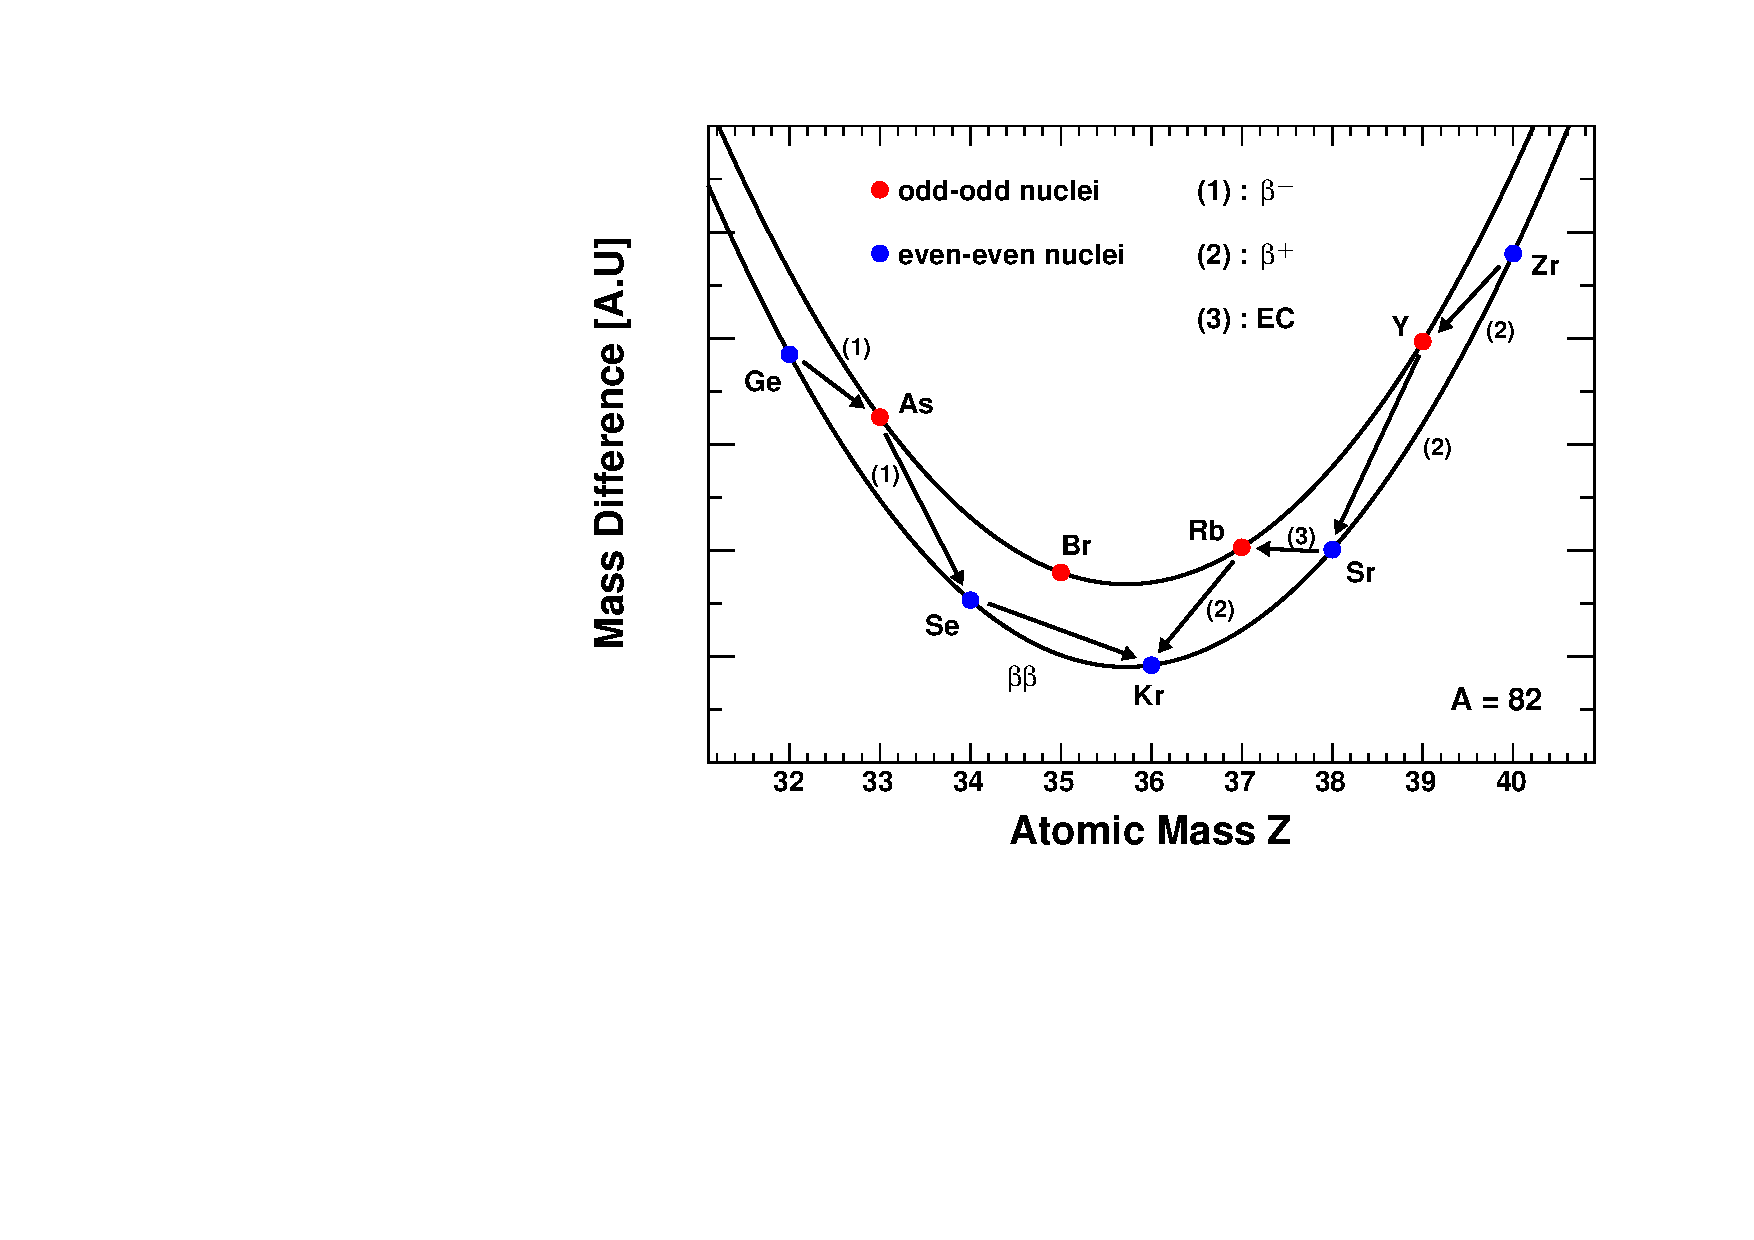
\includegraphics[scale=0.6]{pictures/Chap2/WeizsackerParabola_v3.pdf}
\caption{Mass excess according the atomic number Z. The odd-odd isotope (a) can decay to the even-even isotope (b) via a $\beta$ decay. This daughter nucleus undergoes a beta decay to reach (c). The isotope (c) can not decay to (d) due to the energy conservation. To become more stable, only a 2$\nu\beta\beta$ decay is possible.}
\label{WeizsackerParabola}
\end{center}
\end{figure}


\FloatBarrier


\section{Two Neutrino Double Beta Decay}\label{sec:2NeutrinoDBD}


\NI The two neutrino double beta decay (2$\nu\beta\beta$~decay) is a rare process in which 2$\beta^{-}$ or 2$\beta^{+}$ decays happens simulataneously~: 


\begin{equation}
\mathcal{N} (\text{A,Z}) \rightarrow \mathcal{N} (\text{A,Z+2}) + \text{2e}^- + \text{2}\bar{\nu}_{\text{e}} 
\end{equation}

\begin{equation}
\mathcal{N} (\text{A,Z}) \rightarrow \mathcal{N} (\text{A,Z-2}) + \text{2e}^+ + \text{2}\nu_{\text{e}} 
\end{equation}


\bigskip


\NI It is a second order process allowed in the Standard Model. Its existence have been proposed by Goeppert-Mayer in 1935~\cite{GoeppertMayerDoubleBetaDecay}. The Feynman diagram of the decay is shown in~Figure~\ref{2nubbFeynman}.

 
\begin{figure}[h!]
\begin{center}
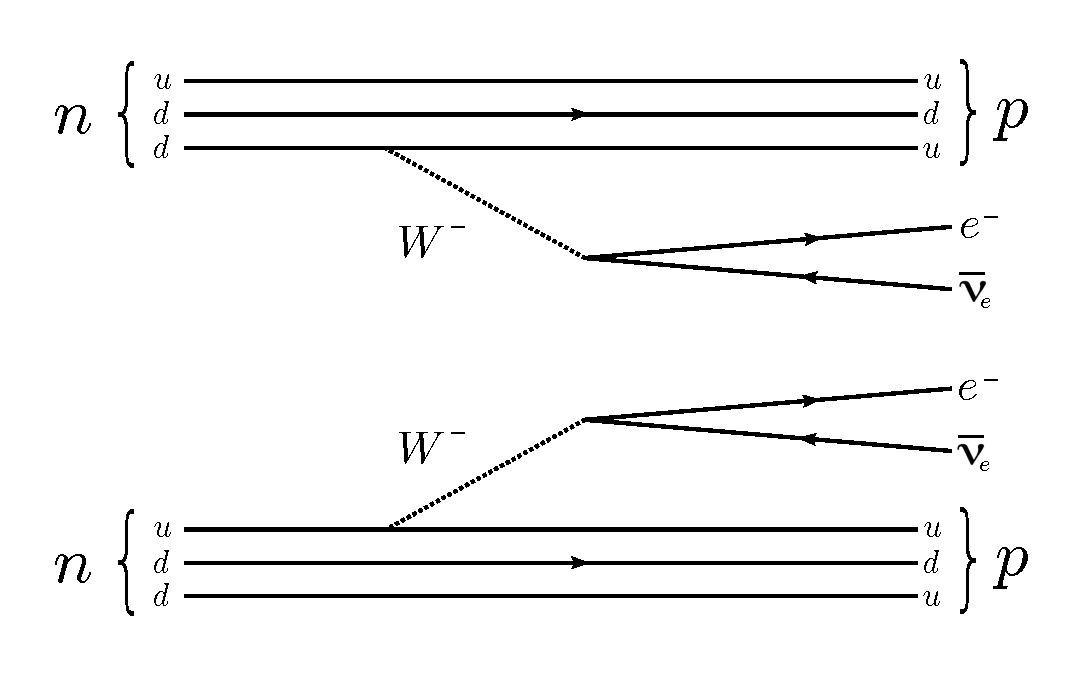
\includegraphics[scale=0.5]{pictures/Chap2/2nubbFeynmanDiagram_v3.pdf}
\caption{Feynman diagram for 2$\nu\beta\beta$ decay. In this second order process, 2 neutrons decay simultaneously (2n $\rightarrow$ 2p + 2e$^-$ + 2$\bar{\nu}$). Two electrons and two anti-neutrinos are emitted.}
\label{2nubbFeynman}
\end{center}
\end{figure}



\bigskip


\NI Since the antineutrinos carry away a part of the energy, the total energy of the emitted electrons is a continuous spectrum with an end-point at the nuclear transition energy, Q$_{\beta\beta}$, defined as :


\begin{equation}
\text{Q}_{\beta\beta} = \mathcal{M}_\text{i} - (\mathcal{M}_\text{f} + \text{2m}_\text{e})
\end{equation}


\bigskip


\NI where m$_\text{e}$ is the electron mass. The shape of this spectrum is shown in Figure~\ref{bbDecaySpectrum}. The half-life of the decay can be written as : 


\begin{equation}
(\text{T}_{\text{1/2}}^{\text{2}\nu})^{\text{-1}} = \text{G}_{\text{2}\nu}(\text{Q}_{\beta\beta}, \text{Z}) \times |\text{M}_{\text{2}\nu}|^\text{2}
\end{equation}


\bigskip


\NI where G$_{\text{2}\nu}$ is the phase space factor that can be well calculated analytically and M$_{\text{2}\nu}$ is the nuclear matrix element (NME) for the decay. The computation of the NME are not trivial and are strongly model-dependent. More details about NME will be given in Section~\ref{sec:NME}.






\NI The 2$\nu\beta\beta$~decay is possible only for the odd-odd nucleus and can also been observed if the spin difference is too huge during the transition (this is the case for $^{\text{48}}$Ca). The double $\beta^{+}$ decays is in competition with the double electron captures. Futhermore, their Q$_{\beta\beta}$ are smaller and their half-lives higher than the double $\beta^{i}$ decays, explaining why these decays are rarely studied. It exists 41 natural isotopes capable of 2$\nu\beta\beta$~decay (35 by double $\beta^{-}$ and 6 by $\beta^{+}$). Their decay rate have been experimentally observed for 12 of them, Table~[] summarized some of their properties.

\section{Neutrinoless Double Beta Decay}\label{sec:0NeutrinoDBD}

\begin{figure}[h!]
\begin{center}
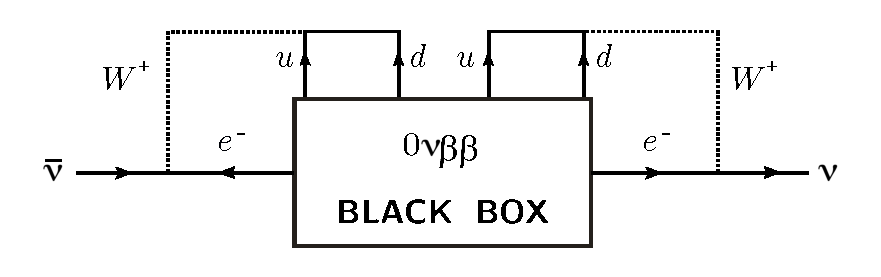
\includegraphics[scale=0.8]{pictures/Chap2/0nubbBlackBox.pdf}
\caption{Feynman diagram for 2$\nu\beta\beta$ decay. In this second order process, 2 neutrons decay simultaneously (2n $\rightarrow$ 2p + 2e$^-$ + 2$\bar{\nu}$). Two electrons and two anti-neutrinos are emitted.}
\label{0nubbBlackBox}
\end{center}
\end{figure}



\begin{table}
\centering
\begin{tabular}{|c|c|c|c|c|}
\hline
Transition & Q$_{\beta\beta}$~keV & $\eta$ [\%] & G$^{\text{2}\nu}$ [y$^{\text{-1}}$] & G$^{\text{0}\nu}$ [y$^{\text{-1}}$] \\
\hline
$^{\text{46}}$Ca $\rightarrow$ $^{\text{46}}$Ti & 987      $\pm$ 4   & 0.035  & 1.148 10$^{\text{-22}}$ & 1.397 10$^{\text{-27}}$\\
\hline
$^{\text{48}}$Ca $\rightarrow$ $^{\text{48}}$Ti & 4272     $\pm$ 4   & 0.187  & 3.968 10$^{\text{-17}}$ & 2.439 10$^{\text{-25}}$\\ 
\hline
$^{\text{70}}$Zn $\rightarrow$ $^{\text{70}}$Ge & 1001     $\pm$ 3   & 0.62   & 3.155 10$^{\text{-22}}$ & 2.342 10$^{\text{-27}}$\\ 
\hline
$^{\text{76}}$Ge $\rightarrow$ $^{\text{76}}$Se & 2039.6   $\pm$ 0.9 & 7.61   & 1.305 10$^{\text{-19}}$ & 2.445 10$^{\text{-26}}$\\ 
\hline
$^{\text{80}}$Se $\rightarrow$ $^{\text{80}}$Kr & 130      $\pm$ 9   & 49.8   & 1.220 10$^{\text{-28}}$ & 4.274 10$^{\text{-29}}$\\ 
\hline
$^{\text{82}}$Se $\rightarrow$ $^{\text{82}}$Kr & 2998     $\pm$ 6   & 8.73   & 4.348 10$^{\text{-18}}$ & 1.079 10$^{\text{-25}}$\\ 
\hline
$^{\text{86}}$Kr $\rightarrow$ $^{\text{86}}$Sr & 1256     $\pm$ 5   & 17.3   & 3.333 10$^{\text{-21}}$ & 6.369 10$^{\text{-27}}$\\ 
\hline
$^{\text{94}}$Zr $\rightarrow$ $^{\text{94}}$Mo & 1145.3   $\pm$ 2.5 & 17.4   & 2.304 10$^{\text{-21}}$ & 6.369 10$^{\text{-27}}$\\ 
\hline
$^{\text{96}}$Zr $\rightarrow$ $^{\text{96}}$Mo & 3350     $\pm$ 3   & 2.8    & 1.927 10$^{\text{-17}}$ & 2.242 10$^{\text{-25}}$\\ 
\hline
$^{\text{98}}$Mo $\rightarrow$ $^{\text{98}}$Ru & 112      $\pm$ 7   & 24.1   & 9.709 10$^{\text{-29}}$ & 6.711 10$^{\text{-29}}$\\ 
\hline
$^{\text{100}}$Mo $\rightarrow$ $^{\text{100}}$Ru & 3034   $\pm$ 6   & 9.63   & 9.434 10$^{\text{-18}}$ & 1.754 10$^{\text{-25}}$\\ 
\hline
$^{\text{104}}$Ru $\rightarrow$ $^{\text{104}}$Pd & 1299   $\pm$ 4   & 18.7   & 9.174 10$^{\text{-21}}$ & 1.202 10$^{\text{-26}}$\\ 
\hline
$^{\text{110}}$Pd $\rightarrow$ $^{\text{110}}$Cd & 2013   $\pm$ 19  & 11.8   & 3.984 10$^{\text{-19}}$ & 5.376 10$^{\text{-26}}$\\ 
\hline
$^{\text{114}}$Cd $\rightarrow$ $^{\text{114}}$Sn & 534    $\pm$ 4   & 28.7   & 1.443 10$^{\text{-23}}$ & 1.639 10$^{\text{-27}}$\\ 
\hline
$^{\text{116}}$Cd $\rightarrow$ $^{\text{116}}$Sn & 2805   $\pm$ 4   & 7.49   & 8.000 10$^{\text{-18}}$ & 1.894 10$^{\text{-25}}$\\ 
\hline
$^{\text{122}}$Sn $\rightarrow$ $^{\text{122}}$Te & 364    $\pm$ 4   & 4.56   & 1.047 10$^{\text{-24}}$ & 8.621 10$^{\text{-28}}$\\ 
\hline
$^{\text{124}}$Sn $\rightarrow$ $^{\text{124}}$Te & 2288   $\pm$ 1.6 & 5.64   & 1.686 10$^{\text{-18}}$ & 1.055 10$^{\text{-25}}$\\ 
\hline
$^{\text{128}}$Te $\rightarrow$ $^{\text{128}}$Xe & 868    $\pm$ 4   & 31.7   & 8.475 10$^{\text{-22}}$ & 6.993 10$^{\text{-27}}$\\ 
\hline
$^{\text{130}}$Te $\rightarrow$ $^{\text{130}}$Xe & 2528.9 $\pm$ 2.1 & 33.8   & 4.808 10$^{\text{-18}}$ & 1.698 10$^{\text{-25}}$\\ 
\hline
$^{\text{134}}$Xe $\rightarrow$ $^{\text{134}}$Ba & 847    $\pm$ 10  & 10.4   & 8.621 10$^{\text{-22}}$ & 7.692 10$^{\text{-27}}$\\ 
\hline
$^{\text{136}}$Xe $\rightarrow$ $^{\text{136}}$Ba & 2479   $\pm$ 8   & 8.9    & 4.831 10$^{\text{-18}}$ & 1.812 10$^{\text{-25}}$\\ 
\hline
$^{\text{142}}$Ce $\rightarrow$ $^{\text{142}}$Nd & 1417.6 $\pm$ 2.5 & 11.1   & 7.246 10$^{\text{-20}}$ & 1.812 10$^{\text{-26}}$\\
\hline 
$^{\text{146}}$Nd $\rightarrow$ $^{\text{146}}$Sm & 56     $\pm$ 5   & 17.2   & 4.854 10$^{\text{-30}}$ & 1.418 10$^{\text{-28}}$\\
\hline 
$^{\text{148}}$Nd $\rightarrow$ $^{\text{148}}$Sm & 1928.3 $\pm$ 1.9 & 5.7    & 1.070 10$^{\text{-18}}$ & 1.276 10$^{\text{-25}}$\\
\hline 
$^{\text{150}}$Nd $\rightarrow$ $^{\text{150}}$Sm & 3368.1 $\pm$ 2.2 & 5.6    & 1.189 10$^{\text{-16}}$ & 8.000 10$^{\text{-25}}$\\ 
\hline
$^{\text{154}}$Sm $\rightarrow$ $^{\text{154}}$Gd & 1251.9 $\pm$ 1.5 & 22.6   & 4.098 10$^{\text{-20}}$ & 4.202 10$^{\text{-26}}$\\ 
\hline
$^{\text{160}}$Gd $\rightarrow$ $^{\text{160}}$Dy & 1729.5 $\pm$ 1.4 & 21.8   & 6.623 10$^{\text{-19}}$ & 1.252 10$^{\text{-25}}$\\ 
\hline
$^{\text{170}}$Gr $\rightarrow$ $^{\text{170}}$Yd & 653.9  $\pm$ 1.6 & 14.9   & 5.495 10$^{\text{-22}}$ & 1.445 10$^{\text{-26}}$\\ 
\hline
$^{\text{176}}$Yb $\rightarrow$ $^{\text{176}}$Hf & 1078.8 $\pm$ 2.7 & 12.6   & 3.067 10$^{\text{-20}}$ & 5.714 10$^{\text{-26}}$\\ 
\hline
$^{\text{186}}$W $\rightarrow$ $^{\text{186}}$Os & 490.3   $\pm$ 2.2 & 28.6   & 1.302 10$^{\text{-22}}$ & 1.439 10$^{\text{-26}}$\\ 
\hline
$^{\text{192}}$Os $\rightarrow$ $^{\text{192}}$Pj & 417    $\pm$ 4   & 41.0   & 5.051 10$^{\text{-23}}$ & 1.299 10$^{\text{-26}}$\\ 
\hline 
$^{\text{198}}$Pt $\rightarrow$ $^{\text{198}}$Hg & 1048   $\pm$ 4   & 7.2    & 6.135 10$^{\text{-20}}$ & 1.144 10$^{\text{-25}}$\\
\hline 
$^{\text{204}}$Hg $\rightarrow$ $^{\text{204}}$Pb & 416.5  $\pm$ 1.9 & 6.9    & 8.130 10$^{\text{-23}}$ & 1.976 10$^{\text{-26}}$\\
\hline 
$^{\text{232}}$Th $\rightarrow$ $^{\text{232}}$U & 858     $\pm$ 6   & 100    & 5.952 10$^{\text{-20}}$ & 2.519 10$^{\text{-25}}$\\
\hline 
$^{\text{238}}$U $\rightarrow$ $^{\text{238}}$Pu & 1145.8  $\pm$ 1.7 & 99.275 & 6.803 10$^{\text{-19}}$ & 5.952 10$^{\text{-25}}$\\ 
\hline
\end{tabular}
\caption{dd}
\end{table}


\FloatBarrier


\subsection{Neutrino Mass Mechanism}


\begin{figure}[h!]
\begin{center}
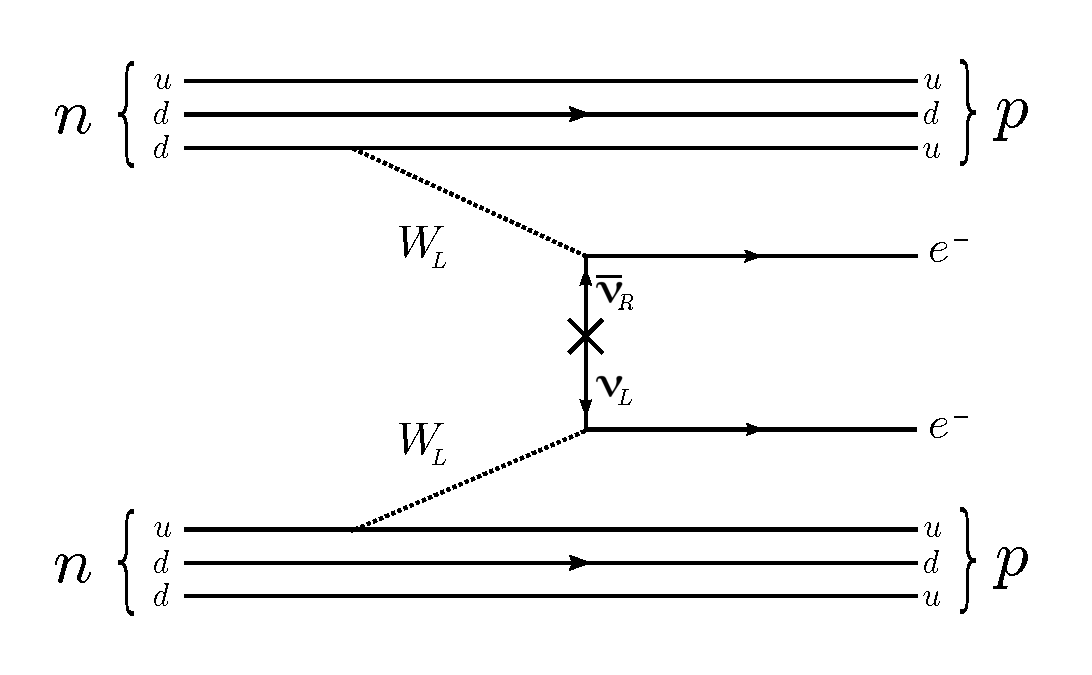
\includegraphics[scale=0.5]{pictures/Chap2/0nubbFeynmanDiagram_NMM.pdf}
\caption{Feynman diagram for 2$\nu\beta\beta$ decay. In this second order process, 2 neutrons decay simultaneously (2n $\rightarrow$ 2p + 2e$^-$ + 2$\bar{\nu}$). Two electrons and two anti-neutrinos are emitted.}
\label{0nubbNMM}
\end{center}
\end{figure}


\begin{figure}[h!]
\begin{center}
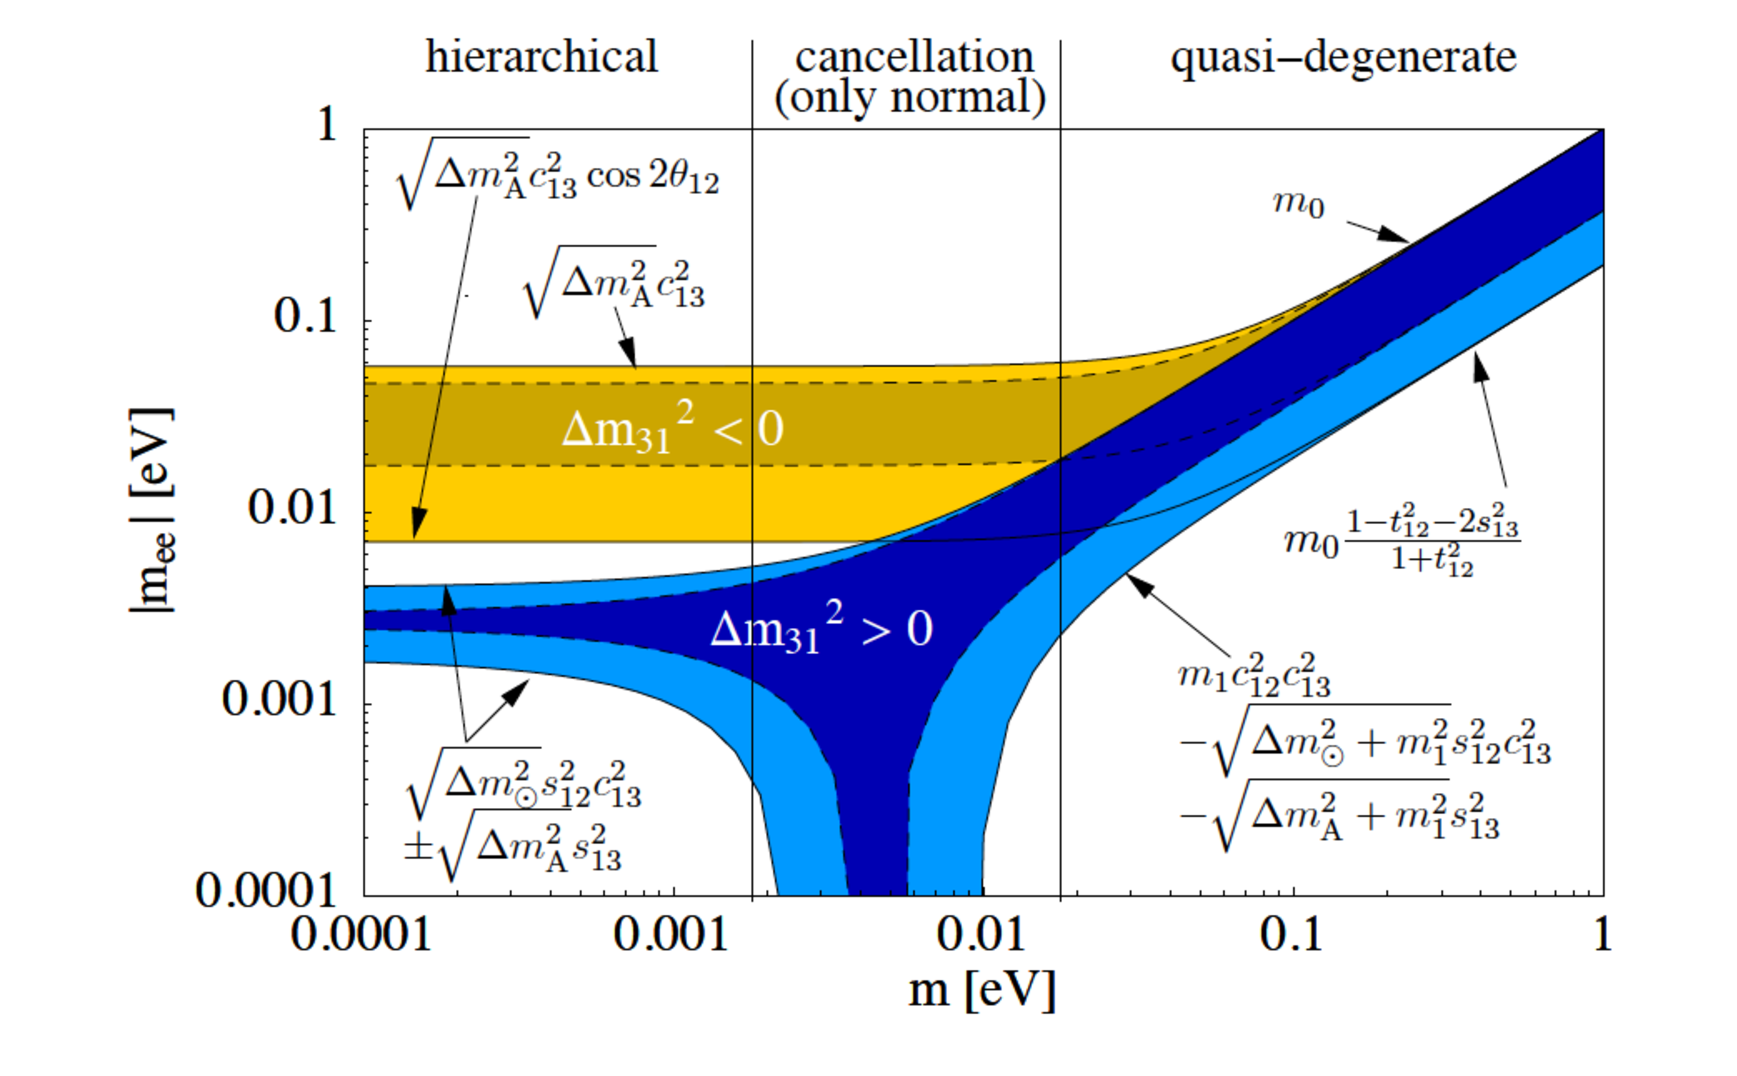
\includegraphics[scale=0.45]{pictures/Chap2/EffectiveMassNMM.pdf}
\caption{Feynman diagram for 2$\nu\beta\beta$ decay. In this second order process, 2 neutrons decay simultaneously (2n $\rightarrow$ 2p + 2e$^-$ + 2$\bar{\nu}$). Two electrons and two anti-neutrinos are emitted.}
\label{EffectiveMassNMM}
\end{center}
\end{figure}


\begin{figure}[h!]
\begin{center}
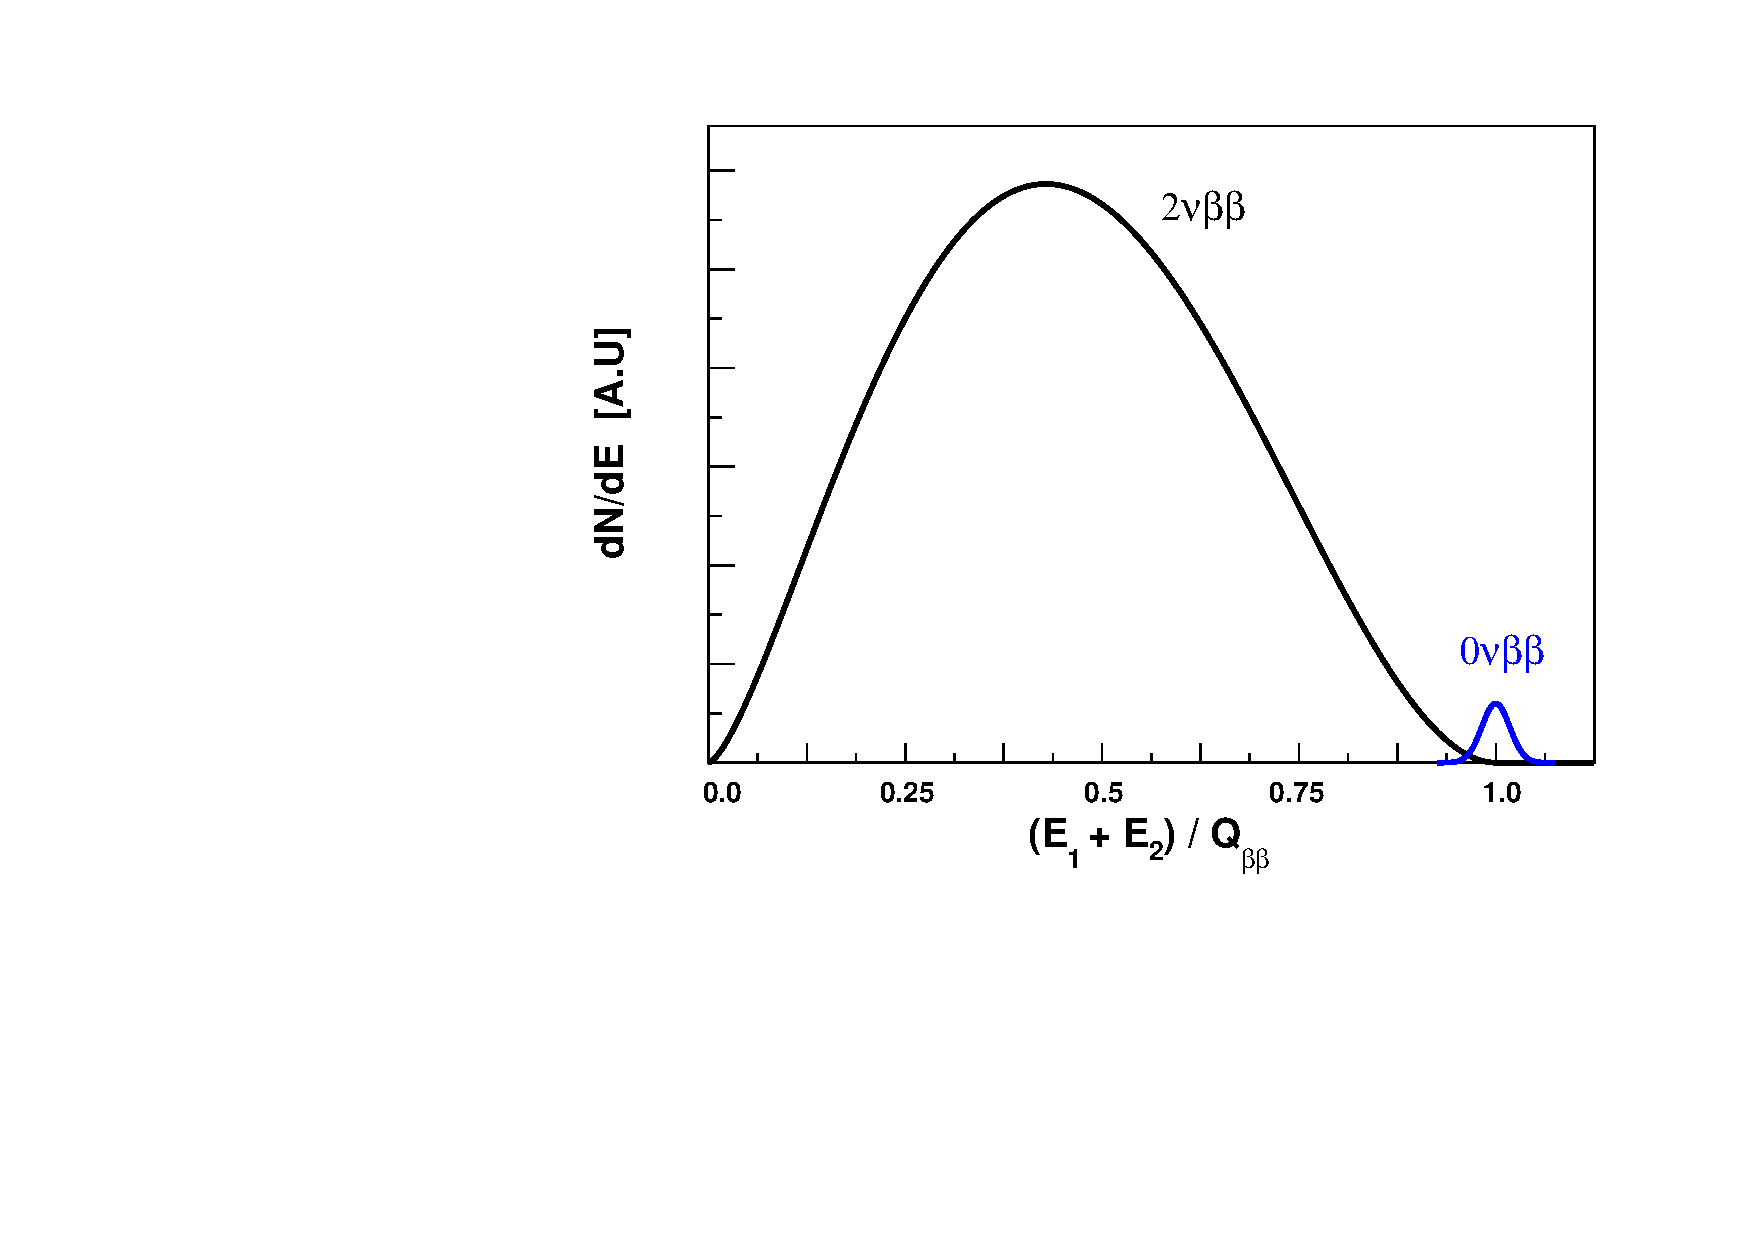
\includegraphics[scale=0.6]{pictures/Chap2/BetaDecaySpectrum.pdf}
\caption{Feynman diagram for 2$\nu\beta\beta$ decay. In this second order process, 2 neutrons decay simultaneously (2n $\rightarrow$ 2p + 2e$^-$ + 2$\bar{\nu}$). Two electrons and two anti-neutrinos are emitted.}
\label{EnergySpectrumDBD}
\end{center}
\end{figure}



\FloatBarrier

\subsection{Other mechanisms}

\subsubsection{Right-handed Current}

\begin{figure}[h!]
\begin{center}
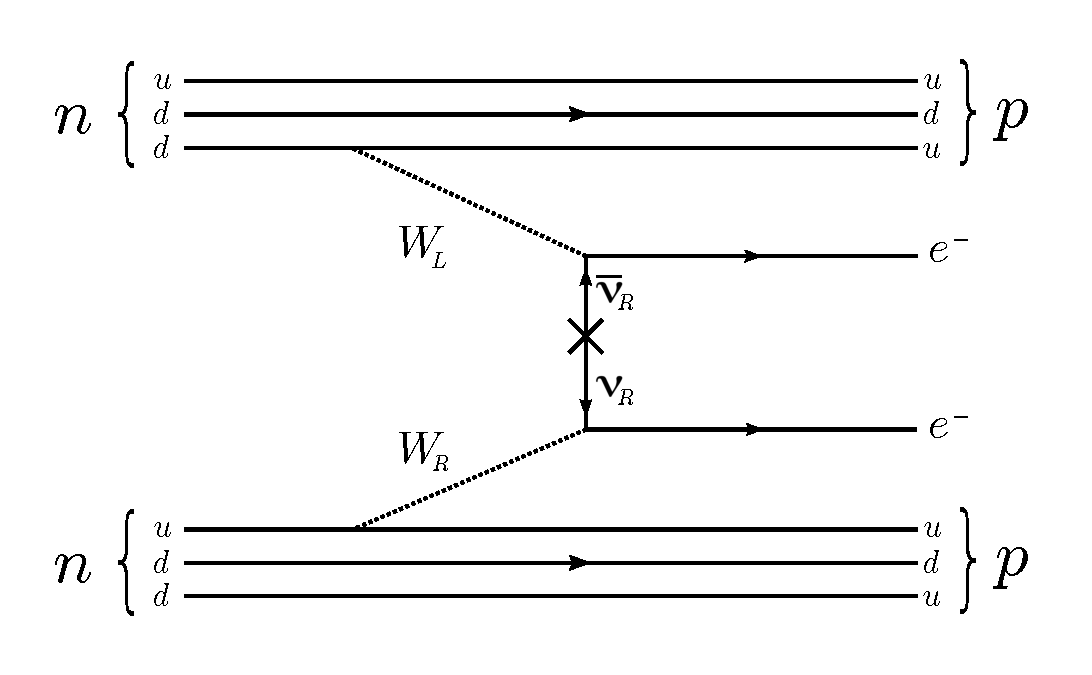
\includegraphics[scale=0.5]{pictures/Chap2/0nubbFeynmanDiagram_RHC.pdf}
\caption{Feynman diagram for 2$\nu\beta\beta$ decay. In this second order process, 2 neutrons decay simultaneously (2n $\rightarrow$ 2p + 2e$^-$ + 2$\bar{\nu}$). Two electrons and two anti-neutrinos are emitted.}
\label{OnbbFeynmanDiagramRHC}
\end{center}
\end{figure}


\begin{figure}[h!]
\begin{center}
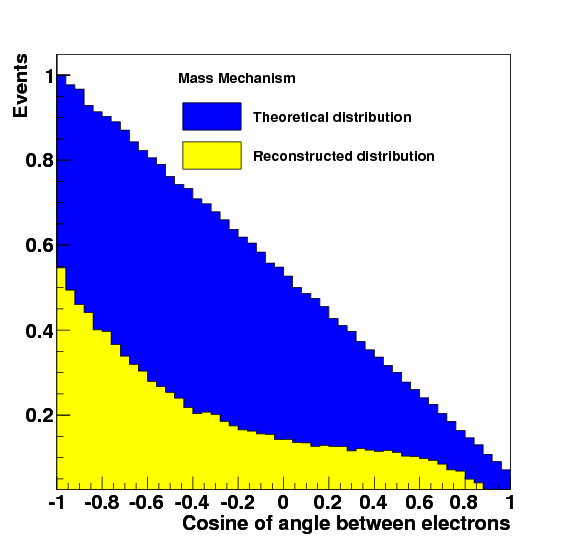
\includegraphics[scale=0.3]{pictures/Chap2/MMcos.png}
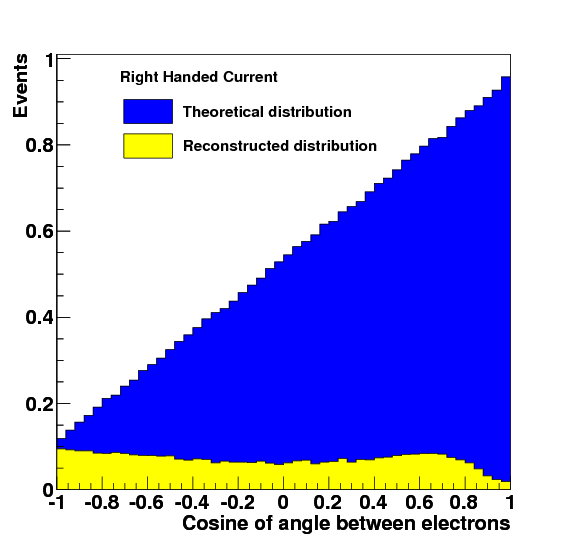
\includegraphics[scale=0.3]{pictures/Chap2/RHCcos.png}
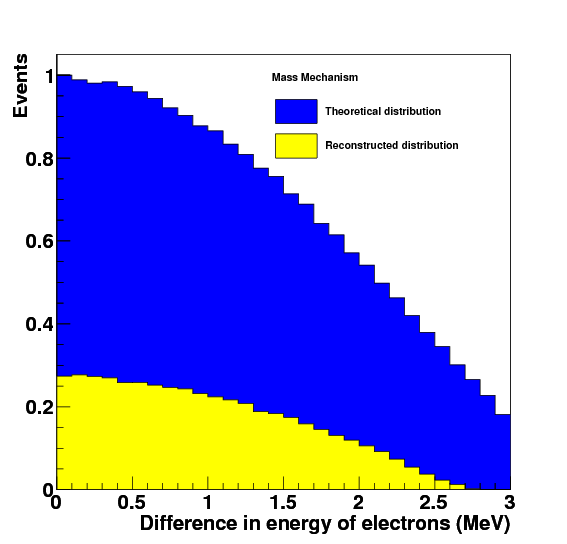
\includegraphics[scale=0.3]{pictures/Chap2/MMenergy.png}
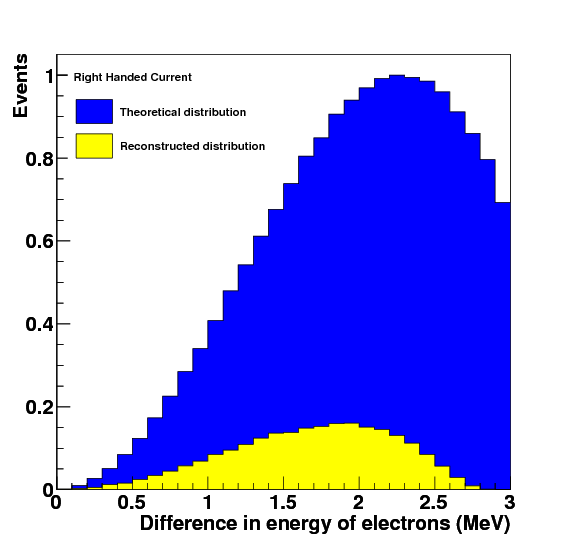
\includegraphics[scale=0.3]{pictures/Chap2/RHCenergy.png}
\caption{Feynman diagram for 2$\nu\beta\beta$ decay. In this second order process, 2 neutrons decay simultaneously (2n $\rightarrow$ 2p + 2e$^-$ + 2$\bar{\nu}$). Two electrons and two anti-neutrinos are emitted.}
\label{TopologyDifferenceNMM-RHC}
\end{center}
\end{figure}



\FloatBarrier

\subsubsection{Majoron Emission}


\begin{figure}[h!]
\begin{center}
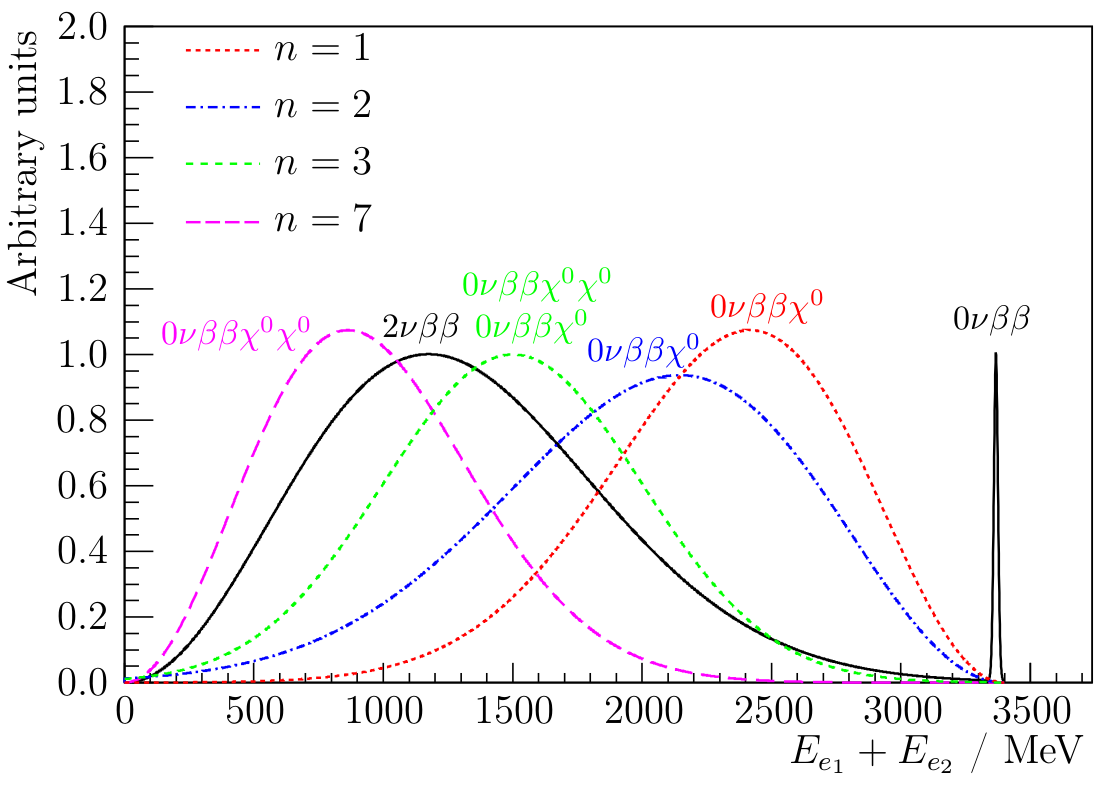
\includegraphics[scale=0.25]{pictures/Chap2/SpectrumFifferentMechanism.png}
\caption{Distribution of the sum of electron energies for 2$\nu\beta\beta$ and 0$\nu\beta\beta$ according different Majoron decay modes with spectal indices 1,2,3 and 7.}
\label{DifferentbbDecaySpectrum}
\end{center}
\end{figure}

\FloatBarrier

\subsubsection{Nuclear Matrix Element}


\begin{figure}[h!]
\begin{center}
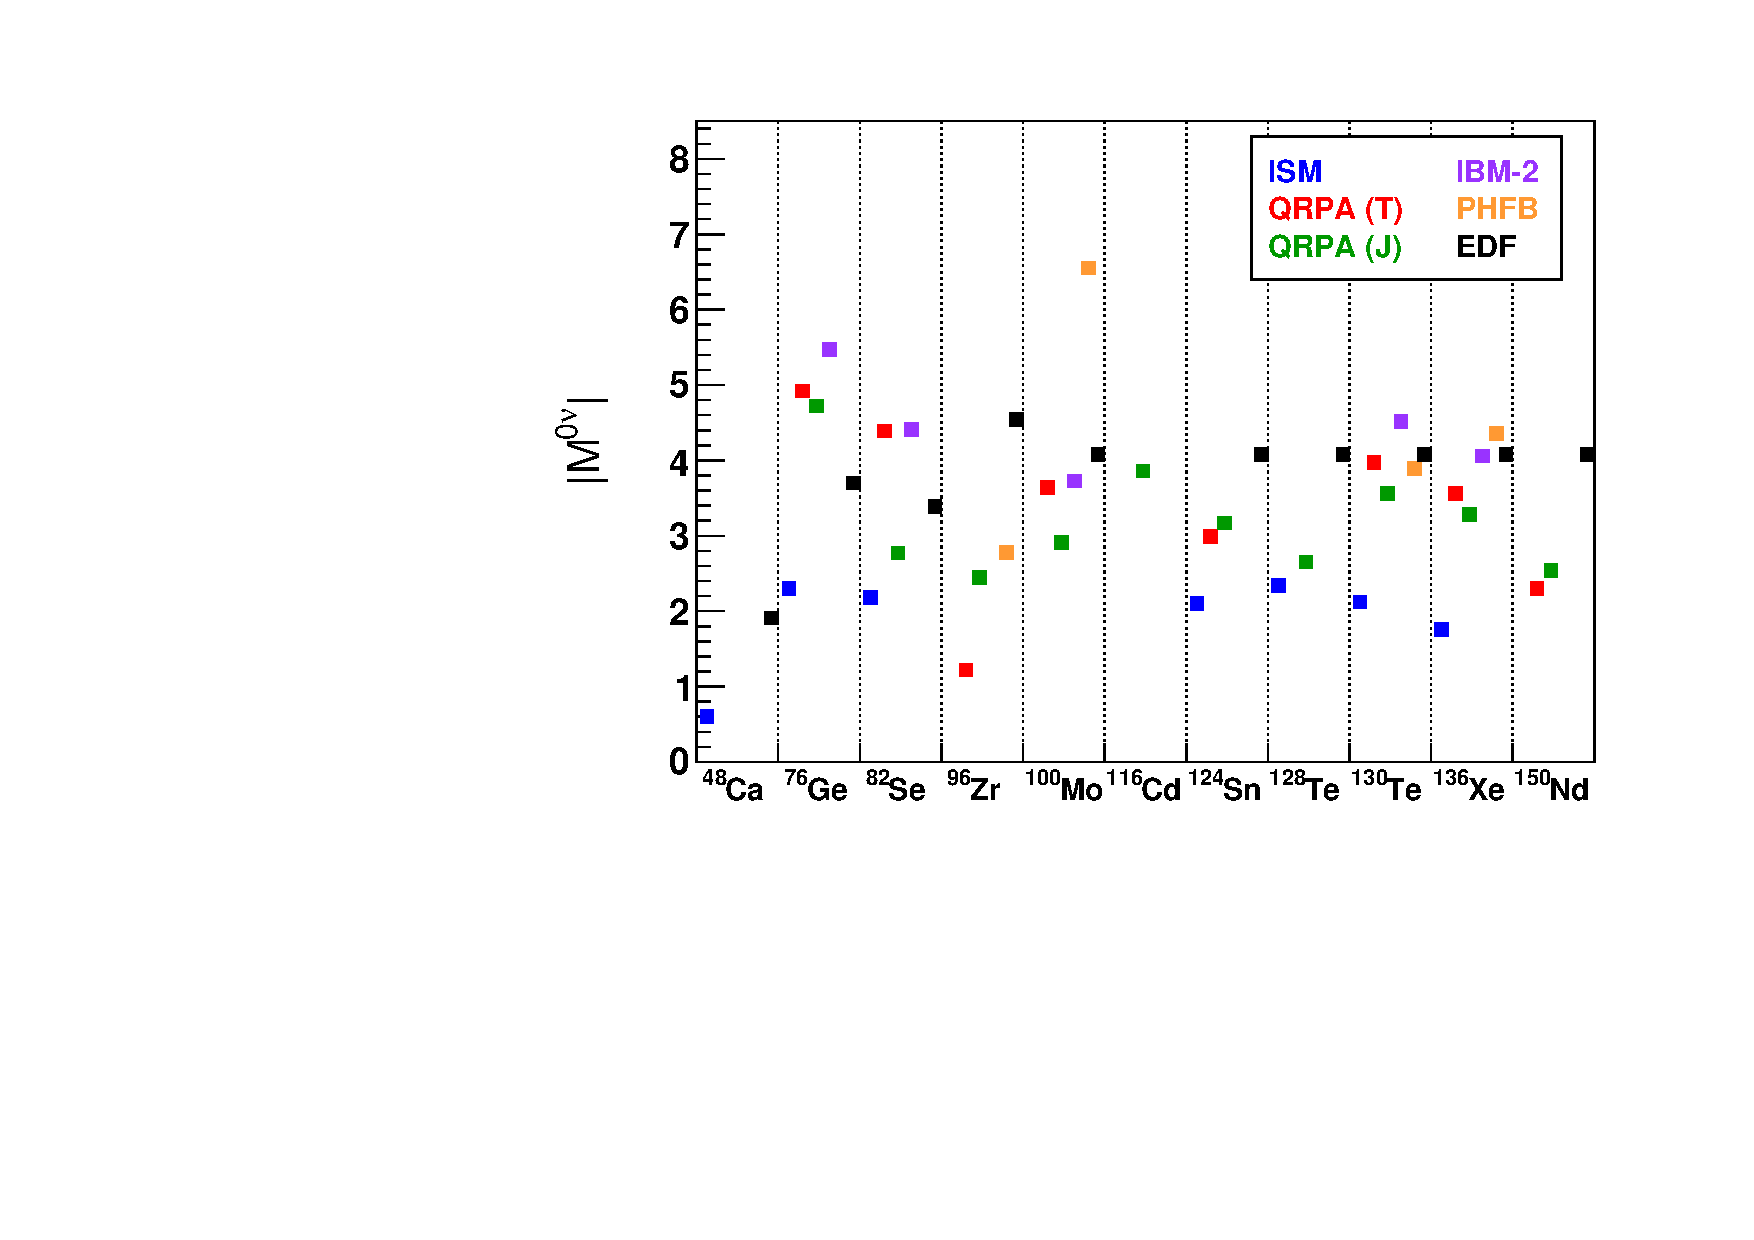
\includegraphics[scale=0.70]{pictures/Chap2/NMEvalue.pdf}
\caption{Summary of 0$\nu\beta\beta$ Nuclear Matrix Element (NME) computations, calculated for 11 isotopes, using different approaches. These results are extracted from \cite{TheoryOfNeutrinolessDBD}, conversion for g$_{\text{A}}$ = 1.25 and r$_{\text{0}}$  = 1.2~fm have been made if necessary.}
\label{NME}
\end{center}
\end{figure}


\FloatBarrier


\section{Double Beta Experiments}\label{sec:DBDexperiment}

\subsection{Half-life sensitivity for 0$\nu\beta\beta$}

\subsection{Maximising signal}

\subsection{Minimising background}

\subsection{Choice of the isotope}

\subsection{Experimental techniques}

HeidelbergMoscow1 \cite{HeidelbergMoscow1} \\
HeidelbergMoscow2 \cite{HeidelbergMoscow2} \\
HeidelbergMoscow3 \cite{HeidelbergMoscow3} \\

IGEX \cite{IGEX} \\
GERDA \cite{GERDA} \\
GERDAprospective \cite{GERDAprospective} \\
MAJORANA \cite{MAJORANA} \\
MAJORANAandGERDA \cite{MAJORANAandGERDA} \\
COBRA \cite{COBRA} \\
ELEGANTVI \cite{ELEGANTVI} \\
CANDLESIII \cite{CANDLESIII} \\
KamLAND-Zen \cite{KamLAND-Zen} \\
KamLAND-Zen2 \cite{KamLAND-Zen2} \\
KamLAND-Zen3 \cite{KamLAND-Zen3} \\

CUORICINO \cite{CUORICINO} \\
CUORE \cite{CUORE} \\
LUCIFER \cite{LUCIFER} \\
EXO-200 \cite{EXO-200} \\
NEXT \cite{NEXT}





\subsubsection{Semiconductor experiments}

\NI \textbf{1. Heidelberg-Moscow experiment}

\bigskip

\NI \textbf{2. IGEX}

\bigskip

\NI \textbf{3. GERDA}

\bigskip

\NI \textbf{4. MAJORANA}

\bigskip

\NI \textbf{5. COBRA}

\subsubsection{Bolometers}

\NI \textbf{6. CUORE}

\subsubsection{Scintillator experiments}

\NI \textbf{7. ELEGANT VI}

\bigskip

\NI \textbf{8. CANDLES III}

\bigskip

\NI \textbf{9. KamLAND-Zen}


\subsubsection{Time projection chambers}

\NI \textbf{10. COBRA}



\section{State of the art and future measurements propects}\label{sec:StatusDBD}


\newpage 



\bigskip



  

\section{The radioactivity}\label{sec:radioactivity}


\NI Discovered in 1896 by Henri Becquerel, while working with phosphorescent materials, and confirmed later by Marie Curie, radioactivity is a physical process in which an unstable isotope loses energy by emitting radiation. Depending on the kind of radiation, the radiative decays have been sorted in 3 types : $\alpha$, $\beta$ and $\gamma$. Radioactivity is a natural phenomenon which can also be provoked (artificial radioactivity).


\bigskip


\NI At the level of a single atom, a radioactive decay is completely random. Even if we know since how long the isotope exist, it is not possible to predict when the decay will occur. But, in case of a collection of atoms, laws of statistics can be applied. The number of remaining (not decayed) isotopes at a certain time, N(t), can be estimated in terms of their decay constant ($\lambda$) or half-life ($\text{t}_{\text{1/2}}$ or T$_{\text{1/2}}$), and N$_\text{0}$, number of atoms in the initial sample : 


\begin{equation}
\text{N(t) = N}_\text{0}~\text{e} ^{-\lambda\text{t}}
\end{equation}


\NI with the relation : T$_{\text{1/2}}$ = ln(2)/$\lambda$. The time elapsed between the initial moment and the moment when it remains half of the initial sample is called the half-life. Half-lives of known isotopes vary widely, from more than 10$^{\text{19}}$ years ($^{\text{209}}$Bi), to 10$^{\text{-23}}$ seconds for highly unstable ones.


\subsubsection{Alpha decay}


\NI Alpha ($\alpha$) decay is a kind of radioactive decay in which an heavy nucleus emits a helium nucleus ($\alpha$ or $^{\text{4}}_{\text{2}}$He), for example, $^{\text{214}}$Po decays to form $^{\text{210}}$Pb :


\begin{equation}
 ^{\text{214}}\text{Po} \rightarrow  ^{\text{210}}\text{Pb} + \alpha
\end{equation} 


\NI Because it is a two-body reaction, the $\alpha$-particle is mono-energetic and at the order of~MeV (Q$_{\alpha}$ = 7.8~MeV in case of $^{\text{214}}$Po). Alpha decay occurs in heavy nuclei and governed by nuclear and electromagnetic interactions. The potential barrier due to the nuclear force is too important to be overcome by the electromagnic force. Only quantum tunnelling allows the emission of an alpha particle by the nucleus.


\subsubsection{Beta decay}




 
\subsubsection{Gamma ($\gamma$) decay}


\NI Just after the $\alpha$ or $\beta$ emission, the nucleus often reach an excited state of the daughter nucleus. It can then decay to a lower energy state by emitting one or more $\gamma$-ray(s). For example, after a $\beta$ decay, $^{\text{60}}\text{Po}$ reaches the excited state of $^{\text{60}}\text{Ni}$ ($^{\text{60}}\text{Ni}^\ast$) which emits 2 $\gamma$-ray at 1.17~MeV and 1.33~MeV : 


\begin{equation}
^{\text{60}}\text{Ni}^\ast \rightarrow ^{\text{60}}\text{Ni} + \gamma~\text{(1.17~MeV)} + \gamma~\text{(1.33~MeV)}
\end{equation}


\NI The emission of a $\gamma$-ray from an excited nucleus is a very fast process (at the order of 10$^{\text{-12}}$ seconds). 


\section{Two neutrino double beta decay}\label{sec:2nubb}


\subsection{Forbidden $\beta$ decays}





\subsection{Phenomenology}





\section{Neutrinoless double beta decay}\label{sec:0nubb}


\NI The neutrinoless double beta decay (0$\nu\beta\beta$) is a hypothesised process proposed by W.H.~Furry in 1939, in which 2$\beta^{-}$ decays occur simultaneously and no neutrino are emitted :


\begin{equation}
\mathcal{N} (\text{A,Z}) \rightarrow \mathcal{N} (\text{A,Z+2}) + \text{2e}^- 
\end{equation}


\bigskip


\NI This decay is forbidden in Standard model because it violates lepton number conservation and have never been observed. As this decay is only possible if neutrino is massive and is a Majorana particle, it constitutes a sensitive method for testing the Majorana nature of neutrinos [ref]. All candidates for 2$\nu\beta\beta$~decay are also candidates for 0$\nu\beta\beta$~decay but, a priori, there is no correlation between the 2 decay rates. 


\bigskip


\NI As no neutrino are emitted, the electrons carry away all the energy. The total energy distribution of the emitted electrons is expected to be peaked at the Q$_{\beta\beta}$ value as shown in Figure~\ref{bbDecaySpectrum}.


\begin{figure}[h!]
\begin{center}
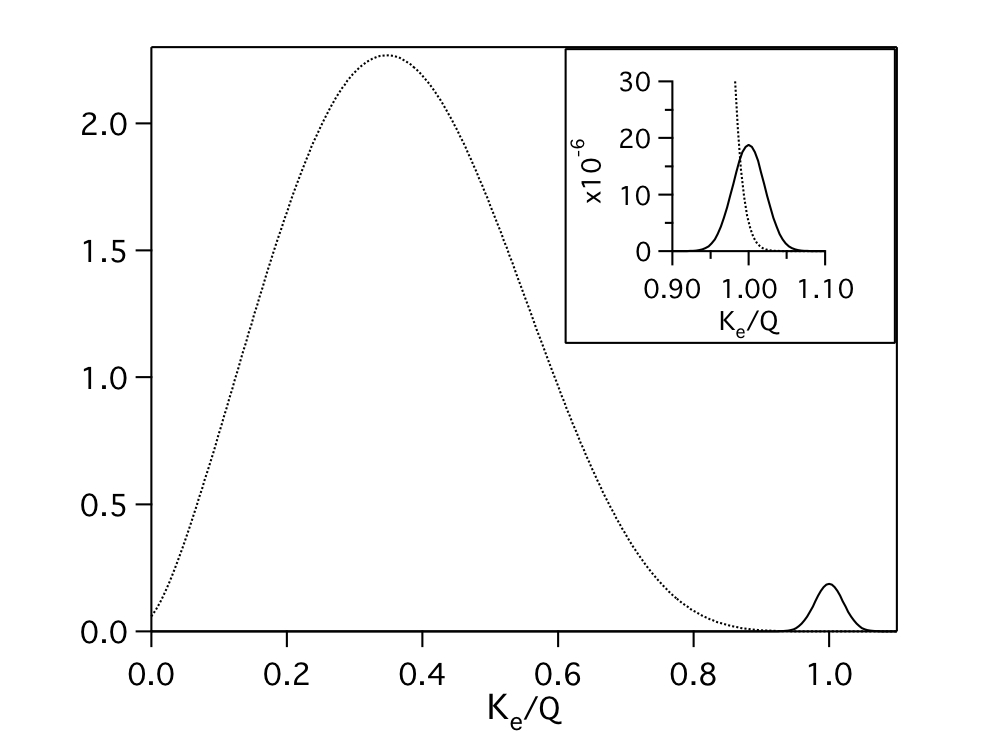
\includegraphics[scale=0.65]{pictures/Chap2/bbspectra.jpg}
\caption{Distribution of the sum of electron energies in case of 2$\nu\beta\beta$ (dashed line) and 0$\nu\beta\beta$ (solid line). The assumptions that $T_{\text{1/2}}^{\text{2}\nu}$ is 1~\% of $T_{\text{1/2}}^{\text{0}\nu}$ and the energy resolution is 2~\% have been done.}
\label{bbDecaySpectrum}
\end{center}
\end{figure}


\NI In the most general case, the half-life of 0$\nu\beta\beta$ is parametrised as : 


\begin{equation}
(\text{T}_{\text{1/2}}^{\text{0}\nu})^{\text{-1}} = \text{G}_{\text{0}\nu}\text{(Q}_{\beta\beta},\text{Z)} \times \text{M}^\text{2}_{\text{0}\nu} \times \eta^\text{2}
\end{equation}


\bigskip


\NI where G$_{\text{0}\nu}$ is a two-body phase space factor unlike G$_{\text{2}\nu}$ which is a four-body phase space factor. This parameter have been computed for different isotopes. M$^\text{2}_{\text{0}\nu}$ is the 0$\nu\beta\beta$ NME, which is not trivial to evaluate due to the high number of nucleons. $\eta$ is a lepton violating number parameter which take into account all the physics behind 0$\nu\beta\beta$ mechanism. This parameter varies according the mechanism via which 0$\nu\beta\beta$ is mediated.  


\bigskip


\NI By trying to draw the Feynman diagram of 0$\nu\beta\beta$ (see Figure~\ref{0nubbFeynman}), 2 problems emerge. The first one concerns the particle-antiparticle difference. The top vertex emits a $\bar{\nu}_{\text{e}}$ which can not be absorbed by the other vertex (absorbing only $\nu_{\text{e}}$). The second one is the helicity difference. The helicity of the lepton emitted by the top vertex is positive and the bottom vertex absorbs only the negative helicity. 


\begin{figure}[h!]
\begin{center}
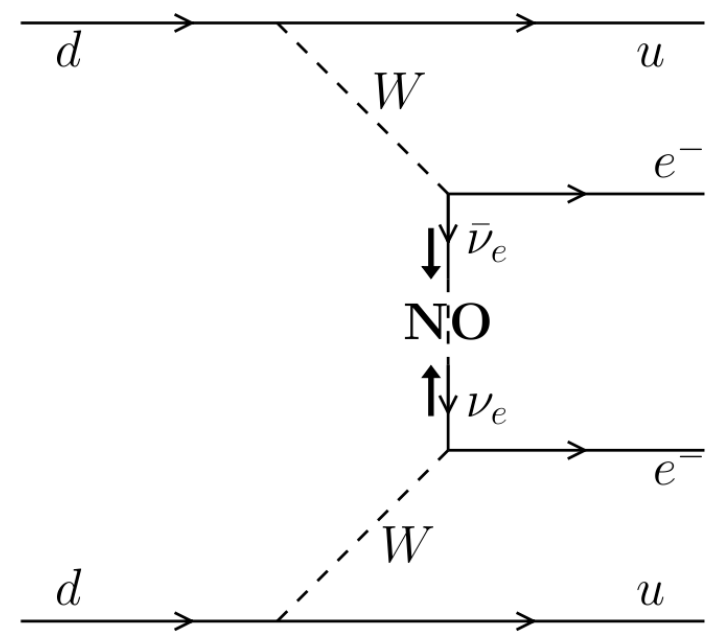
\includegraphics[scale=0.25]{pictures/Chap2/0nubb_Feynman.png}
\caption{Feynman diagram for 0$\nu\beta\beta$ decay. This process is forbidden in Standard Model because of the lepton number violation and have never been observed.}
\label{0nubbFeynman}
\end{center}
\end{figure}


\NI To make possible the 0$\nu\beta\beta$ decay, a change of helicity must occur, which implies a non-zero mass for neutrino and the neutrino has to be a Majorana particle ($\bar{\nu}_{\text{e}}$ = $\nu_{\text{e}}$).


\subsection{Effective mass of Majorana}


\NI The most commonly decay mode and which deviates the least from the SM is the neutrino mass mechanism. In this mechanism, 0$\nu\beta\beta$ is mediated by the light neutrino exchange. A Feynman diagram using only SM vertices can be drawn (Figure~\ref{0nubbFeynmanMassMechanism}), a right helicity Majorana neutrino is emitted from a W boson and absorbed by another as a left helicity Majorana neutrino. The $\eta$ parameter is given by the effective neutrino mass (m$_{\beta\beta}$) and the half-life can be expressed : 


\begin{equation}
(\text{T}_{\text{1/2}}^{\text{0}\nu})^{\text{-1}} = \text{G}_{\text{0}\nu}\text{(Q}_{\beta\beta},\text{Z)} \times \text{M}^\text{2}_{\text{0}\nu} \times \left( \frac{\text{m}_{\beta\beta}}{\text{m}_\text{e}} \right)^\text{2}
\end{equation}


\bigskip


\NI where m$_\text{e}$ is the electron mass, and m$_{\beta\beta}$ can be written as a function of PMNS matrix element and neutrino masses (m$_\nu\text{\i}$) : 


\begin{equation}
\begin{split}
\text{m}_{\beta\beta} & = |\sum_\text{i}U_{\text{ei}}^\text{2}~\text{m}_{\nu_\text{i}} | \\
 & = \text{cos}^\text{2}\theta_{\text{12}}~\text{cos}^\text{2}\theta_{\text{13}}~\text{m}_\text{1} + \text{sin}^\text{2}\theta_{\text{12}}~\text{cos}^\text{2}\theta_{\text{13}}~\text{e}^{\text{2i}\lambda_\text{1}} ~\text{m}_\text{2} + \text{sin}^\text{2}\theta_{\text{13}}~\text{e}^{\text{2i}(\lambda_\text{2}-\delta)}~\text{m}_\text{3}
\end{split}
\end{equation}


\bigskip


\NI where $\theta_{\text{12}}$ and $\theta_{\text{13}}$ are the mixing angles of PMNS matrix, $\delta$ is the CP-violating phase, and $\lambda_\text{1}$ and $\lambda_\text{2}$ the Majorana phases.  


\begin{figure}[h!]
\begin{center}
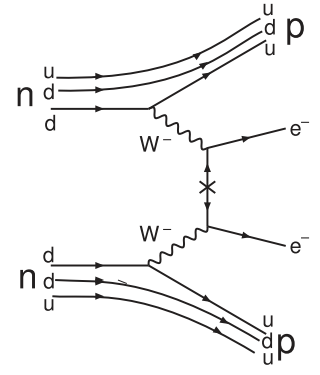
\includegraphics[scale=0.50]{pictures/Chap2/0nubbFeynmanMassMechanism.png}
\caption{Feynman diagram of 0$\nu\beta\beta$ decay in case of light Majorana neutrino exchange. The emitted electron carry over all the energy, the experimental signature is given by a peaked distribution at the Q$_{\beta\beta}$ value.}
\label{0nubbFeynmanMassMechanism}
\end{center}
\end{figure}


\NI The available values for m$_{\beta\beta}$ as a function of the lightest neutrino mass using the best fit values of oscillation parameters are plotted in~Figure~\ref{MeffVsMmin}. It is interesting to note that neutrino oscillation experiments do not give access to the neutrino nature or mass scale but are intimately linked with 0$\nu\beta\beta$ searches via m$_{\beta\beta}$. The green and blue bands represent the reachable values for m$_{\beta\beta}$ in case of normal and inverted ordering of neutrino mass. The width of each of these bands is mainly governed by the uncertainty over the CP-violating phase. The 0$\nu\beta\beta$ experiments put limit on m$_{\beta\beta}$ (y-axis), during direct (Katrin) and indirect (cosmology) could set limit on the lighest neutrino mass (x-axis). The coming 0$\nu\beta\beta$ projects could probe the inverted ordering area with real prospects for either observing of excluding 0$\nu\beta\beta$ mediated by the mass mechanism (in case nature chosen the inverted ordering).


\begin{figure}[h!]
\begin{center}
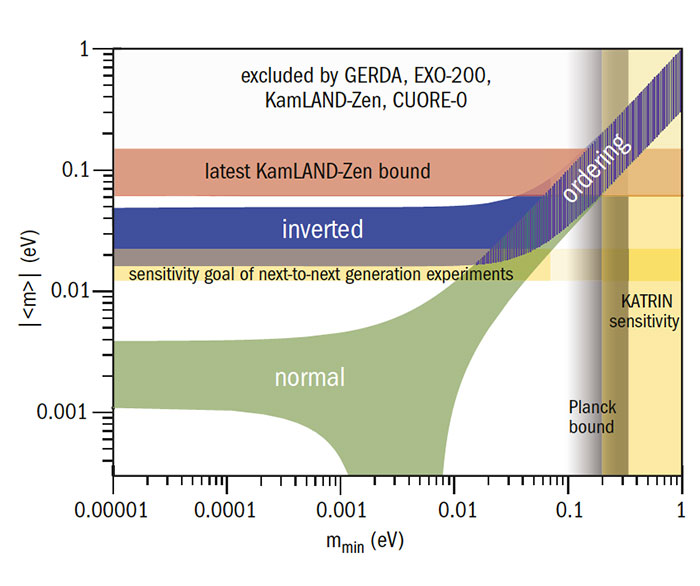
\includegraphics[scale=0.60]{pictures/Chap2/MeffVsMmin.jpg}
\caption{aaa}
\label{MeffVsMmin}
\end{center}
\end{figure}


\FloatBarrier

\subsection{Other processes behond $\beta\beta0\nu$}


\NI For now, I only discussed that the 0$\nu\beta\beta$ decay could be due to an exchange of light neutrino but it exists many  other different mechanisms. All these mechanisms imply new interactions or/and new particles beyond the SM. The most common and quoting most in the literature are the right-handed current and Majoron emission modes. Other more exotic processes as R-parity violating super-symmetry, extra dimensions or squart mixing have also been proposed.


\bigskip


\NI Contrary to the light neutrino exchange mechanism, where the Majorana nature of the neutrino is quite clear, it is not completely obvious for other mechanisms (and in particular for mechanism where neutrino are not involved as in R-parity violating SUSY~[ref]). In 1980, Schechter and Valle proved, thanks to the "black theorem" (Figure~\ref{blackBox}), that whatever the mechanism beyong 0$\nu\beta\beta$ it necessarily involves Majorana neutrino.


\begin{figure}[h!]
\begin{center}
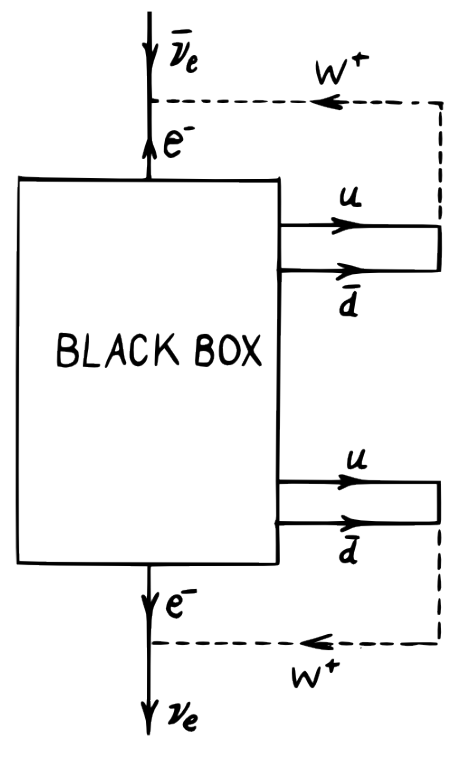
\includegraphics[scale=0.30]{pictures/Chap2/blackBox.png}
\caption{Black box showing that whatever the process behond the 0$\nu\beta\beta$ decay, its observation involves Majorana neutrinos.}
\label{blackBox}
\end{center}
\end{figure}


\FloatBarrier


\NI Un petit mot sur right handed current


\bigskip


\NI Un petit mot sur Majoron


\bigskip


\NI According the considered model, the final topology of the events are different. If one day 0$\nu\beta\beta$ is observed, the measurement of the total energy of the emitted electrons and the angle between them could allow the discrimination between the different mechanisms. Figure~\ref{DifferentbbDecaySpectrum} presented the distribution of total energy electrons according different decays.







\FloatBarrier


\subsection{Nuclear matrix elements}\label{sec:NME}


\NI 



\begin{figure}[h!]
\begin{center}
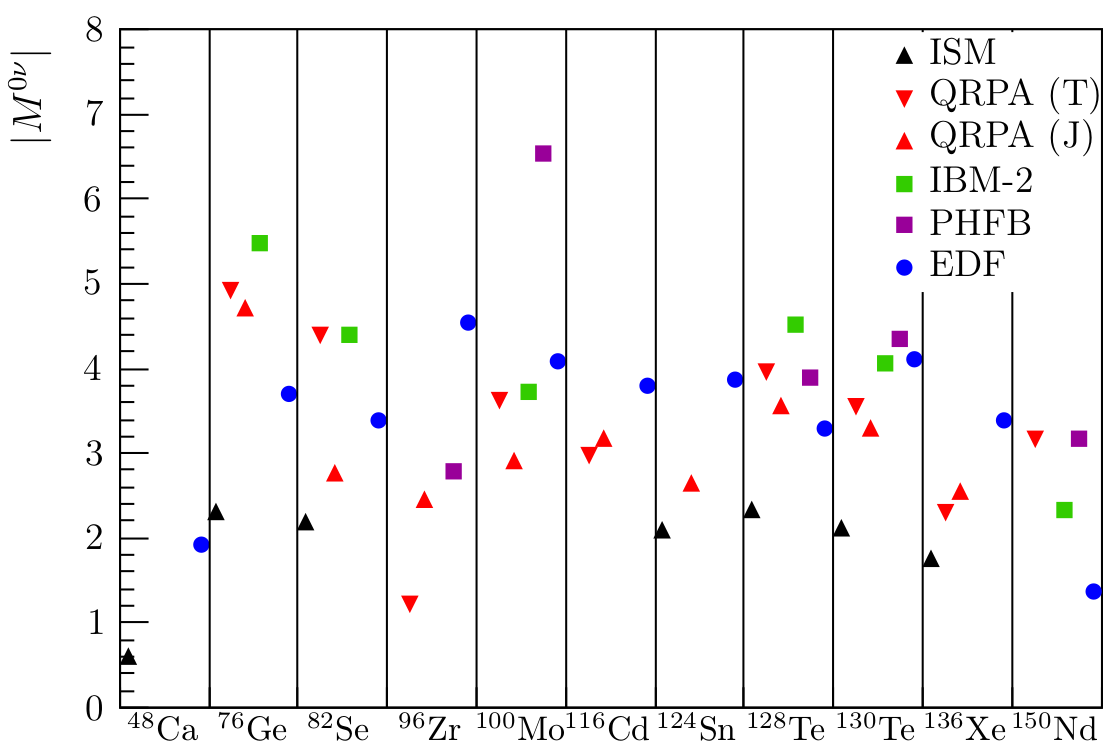
\includegraphics[scale=0.30]{pictures/Chap2/NMEdetailes.png}
\caption{Summary of 0$\nu\beta\beta$ Nuclear Matrix Element (NME) computations, calculated for 11 isotopes, using different approaches. These results are extracted from \cite{TheoryOfNeutrinolessDBD}, conversion for g$_{\text{A}}$ = 1.25 and r$_{\text{0}}$  = 1.2~fm have been made if necessary.}
\label{NME}
\end{center}
\end{figure}


\FloatBarrier


\subsection{Different isotopes}


\NI It exists 41 naturally isotopes capable of 2$\nu\beta\beta$~decay (35 of $\beta^{-}$ and 6 of $\beta^{+}$ decays). Today 12 isotopes have been experimentally observed undergoing 2$\nu\beta\beta$~decay. \textcolor{red}{dire que c'est un émetteru alpha avec une longue demi vie et que la double beta est possible}


\subsubsection{$^{\text{48}}$Ca}


\NI $^\text{48}$Ca is a rare isotope of calcium containing 20 protons and 28 neutrons. It is the lightest nucleus capable of 2$\nu\beta\beta$~decay. It can be considered as the golden isotope for $\beta\beta$ searches since it possesses the higher Q$_{\beta\beta}$ value (Q$_{\beta\beta}$ = 4.3~MeV) which is above almost all backgrounds. Unfortunately, its very low natural abundance (0.187~\%) limit its study at large exposure. Its 2$\nu\beta\beta$~decay rate have been measured by the NEMO-3 detector : T$_{\text{1/2}}^{\text{2}\nu}$ = 6.4 $^{\text{+0.7}}_{\text{-0.6}}$ (stat.) $^{\text{+1.2}}_{\text{-0.9}}$ (syst.) $\times$ 10$^{\text{19}}$ years. 

 
\subsubsection{$^{\text{76}}$Ge}


\NI $^\text{76}$Ge is an isotope of germanium containing 32 protons and 44 neutrons. Its natural abundance is approximately of 7~\%. Its low Q$_{\beta\beta}$ value (Q$_{\beta\beta}$ = 2.029~MeV) can be troublesome for the $\beta\beta$ searches. Its 2$\nu\beta\beta$~decay rate have been measured by the GERDA detector~:~T$_{\text{1/2}}^{\text{2}\nu}$ = 1.926 $\pm$ 0.094 $\times$ 10$^{\text{21}}$ years.   


\subsubsection{$^{\text{78}}$Kr}


\NI $^\text{78}$Kr is an isotope of krypton containing 36 protons and 42 neutrons. Its natural abundance is 0.36~\% . Its 2$\nu\beta\beta$~decay rate have been measured by the Baksan experiment~:~T$_{\text{1/2}}^{\text{2}\nu}$ = 9.2 $^{\text{+5.5}}_{\text{-2.6}}$ $\pm$ 1.3 $\times$ 10$^{\text{21}}$~years.   


\subsubsection{$^{\text{82}}$Se}


\NI $^\text{82}$Se is an isotope of selenium containing 34 protons and 48 neutrons. Its natural abundance is 8.82~\% and its Q$_{\beta\beta}$ value is 2.995~MeV. Its 2$\nu\beta\beta$~decay rate have been measured by the NEMO-3 detector~:~T$_{\text{1/2}}^{\text{2}\nu}$ = 10.07 $\pm$ 0.14 $\pm$ 0.54 $\times$ 10$^{\text{19}}$~years. 


\subsubsection{$^{\text{96}}$Zr}


\NI $^\text{96}$Zr is an isotope of zirconium containing 40 protons and 56 neutrons. Its natural abundance is 2.80~\% and its Q$_{\beta\beta}$ value is 3.348~MeV. Its 2$\nu\beta\beta$~decay rate have been measured by the NEMO-3 detector~:~T$_{\text{1/2}}^{\text{2}\nu}$ = 2.35 $\pm$ 0.14 $\pm$ 0.16 $\times$ 10$^{\text{19}}$~years.


\subsubsection{$^{\text{100}}$Mo}


\NI $^\text{100}$Mo is an isotope of molybdenium containing 40 protons and 56 neutrons. Its natural abundance is 9.74~\% and its Q$_{\beta\beta}$ value is 3.04~MeV. Its 2$\nu\beta\beta$~decay rate have been measured by the NEMO-3 detector~:~T$_{\text{1/2}}^{\text{2}\nu}$ = 7.1 $\pm$ 0.5 $\times$ 10$^{\text{18}}$~years and Ge coincidence~:~6.9 $^{\text{+1.0}}_{\text{-0.8}}$ $\pm$ 0.7 $\times$ 10$^{\text{18}}$~years.


\subsubsection{$^{\text{116}}$Cd}


\NI $^\text{116}$Cd is an isotope of cadmium containing 48 protons and 68 neutrons. Its natural abundance is 7.51~\% and its Q$_{\beta\beta}$ value is 2.809~MeV. Its 2$\nu\beta\beta$~decay rate have been measured by the NEMO-3 detector~:~T$_{\text{1/2}}^{\text{2}\nu}$ = 2.74 $\pm$ 0.04 $\pm$ 0.18 $\times$ 10$^{\text{19}}$~years and by Elegant : 2.6 $^{\text{+0.9}}_{\text{-0.5}}$ $\times$ 10$^{\text{18}}$~years.


\subsubsection{$^{\text{128}}$Te}


\NI $^\text{128}$Te is an isotope of tellerium containing 52 protons and 76 neutrons. Its natural abundance is 31.74~\% and its Q$_{\beta\beta}$ value is 0.867. Its 2$\nu\beta\beta$~decay rate have been measured by geochemical method~:~T$_{\text{1/2}}^{\text{2}\nu}$ = 2.2 $\times$ 10$^{\text{24}}$~years which is the longest half-life of all isotopes proven to be radioactive.


\subsubsection{$^{\text{130}}$Te}


\NI $^\text{130}$Te is an isotope of tellerium containing 52 protons and 78 neutrons. Its natural abundance is 34.08~\% and its Q$_{\beta\beta}$ value is 2.528~MeV. Its most precise measurement of 2$\nu\beta\beta$~decay rate have been measured by CUORE-0~:~T$_{\text{1/2}}^{\text{2}\nu}$ = 8.2 $\pm$ 0.2 $\pm$ 0.6 $\times$ 10$^{\text{20}}$~years.


\subsubsection{$^{\text{136}}$Xe}


\NI $^\text{136}$Xe is an isotope of xenon containing 54 protons and 82 neutrons. Its natural abundance is 8.8573~\% and its Q$_{\beta\beta}$ value is 2.458~MeV. Its 2$\nu\beta\beta$~decay rate have been measured by EXO-200~:~T$_{\text{1/2}}^{\text{2}\nu}$ = 2.165 $\pm$ 0.016 $\pm$ 0.059 $\times$ 10$^{\text{20}}$~years.


\subsubsection{$^{\text{150}}$Nd}


\NI $^\text{150}$Nd is an isotope of neodynium containing 60 protons and 90 neutrons. Its natural abundance is 5.6~\% and its Q$_{\beta\beta}$ value is 3.367~MeV. Its 2$\nu\beta\beta$~decay rate have been measured by NEMO-3~:~T$_{\text{1/2}}^{\text{2}\nu}$ = 9.34 $\pm$ 0.22 $^{\text{+0.62}}_{\text{-0.60}}$ $\times$ 10$^{\text{18}}$~years.


\subsubsection{$^{\text{238}}$U}
\NI 









\FloatBarrier


\section{Experimental point of view}\label{sec:ExperimentalSearches}
\NI mettre formule sens, il faut des détecteurs bas bruit de fond, ... radiopureté ... parler de l'efficacité,
\NI deux approches sont aujourd'hui considérés : tracko calo et juste calo. Point fort et point faible de chaque approche


\FloatBarrier

\section{Status of double beta experiments}\label{sec:Status0nubb}
\NI Faire un statut de la double beta aujourd'hui avec 
\NI Gerda, KamLandZen, Cuore.
\subsection{KamLAND-Zen}
\subsection{GERDA}
\subsection{Cuore}

\begin{figure}[h!]
\begin{center}
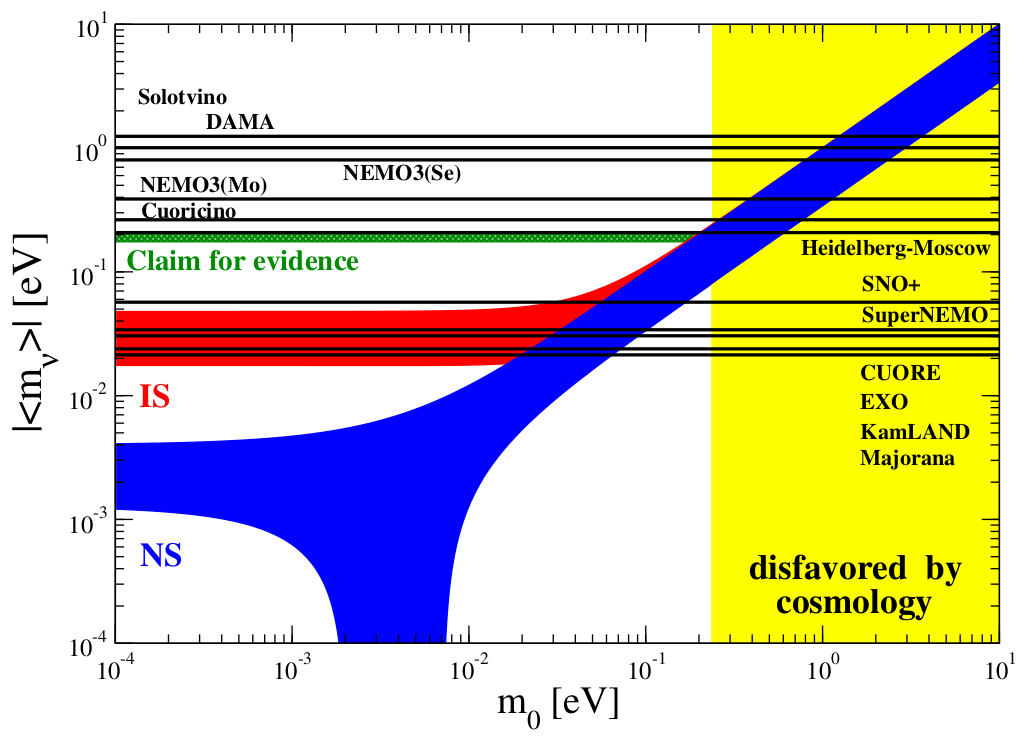
\includegraphics[scale=0.30]{pictures/Chap2/m_eff_neutrino.png}
\caption{Effective neutrino mass (|<m$_{\nu}$>| = m$_{\text{eff}}$) as a function of the lowest mass eigenstate (m$_\text{0}$). The blue and red regions represent the allowed values in Normal and Inverted Spectrum neutrino mass. The current experimental limits are also shown.}
\label{mEff}
\end{center}
\end{figure}









 




\end{document}
